% Editable native annotations around unchanged verified IDE photographs.
\par
\begin{figure}[htbp]
  \centering
  \newsavebox{\MARSwavcandidateregistersBox}
  \sbox{\MARSwavcandidateregistersBox}{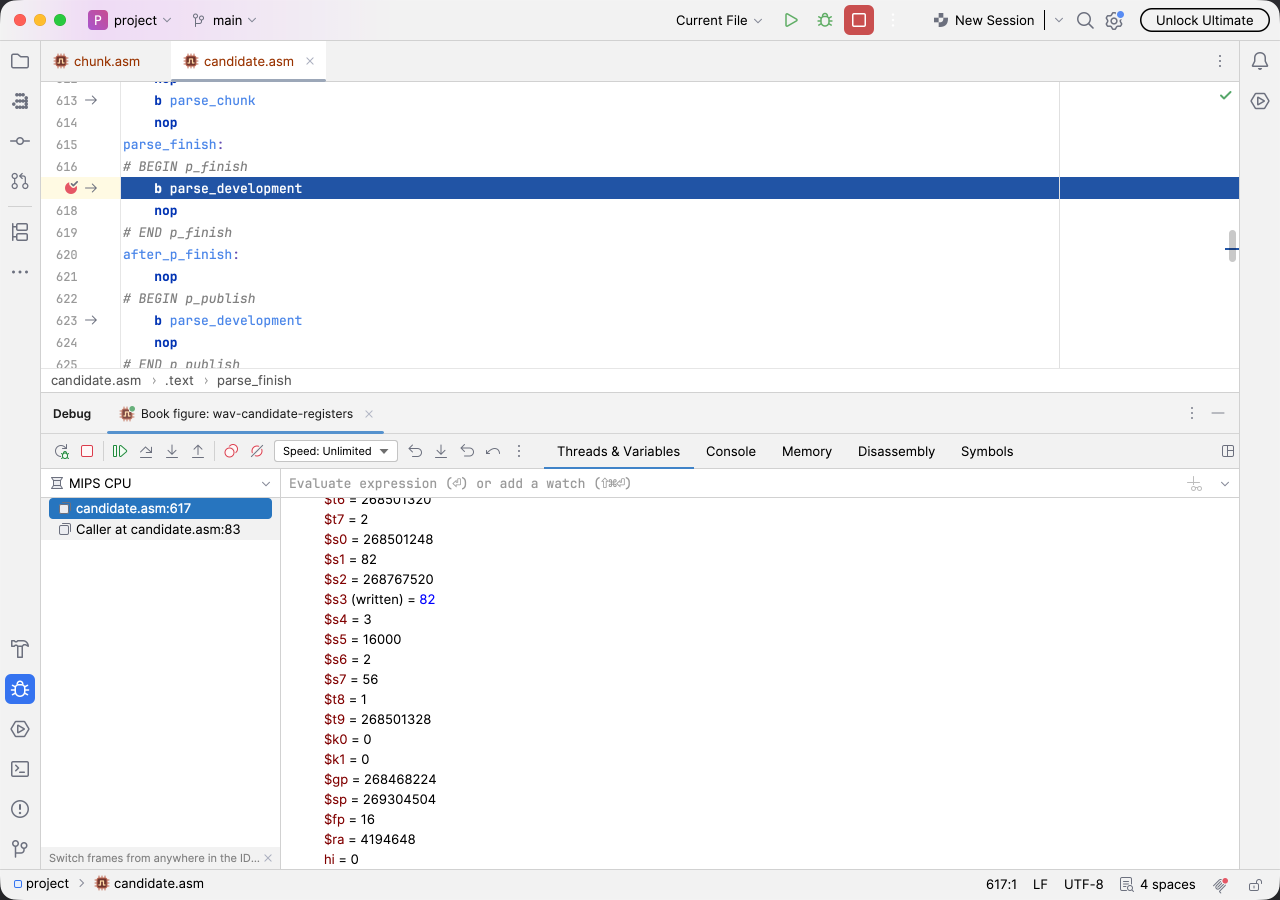
\includegraphics[artifact]{packages/031-pcm-wav/captures/f03/registers.png}}
  \newsavebox{\MARSwavcandidateprivateBox}
  \sbox{\MARSwavcandidateprivateBox}{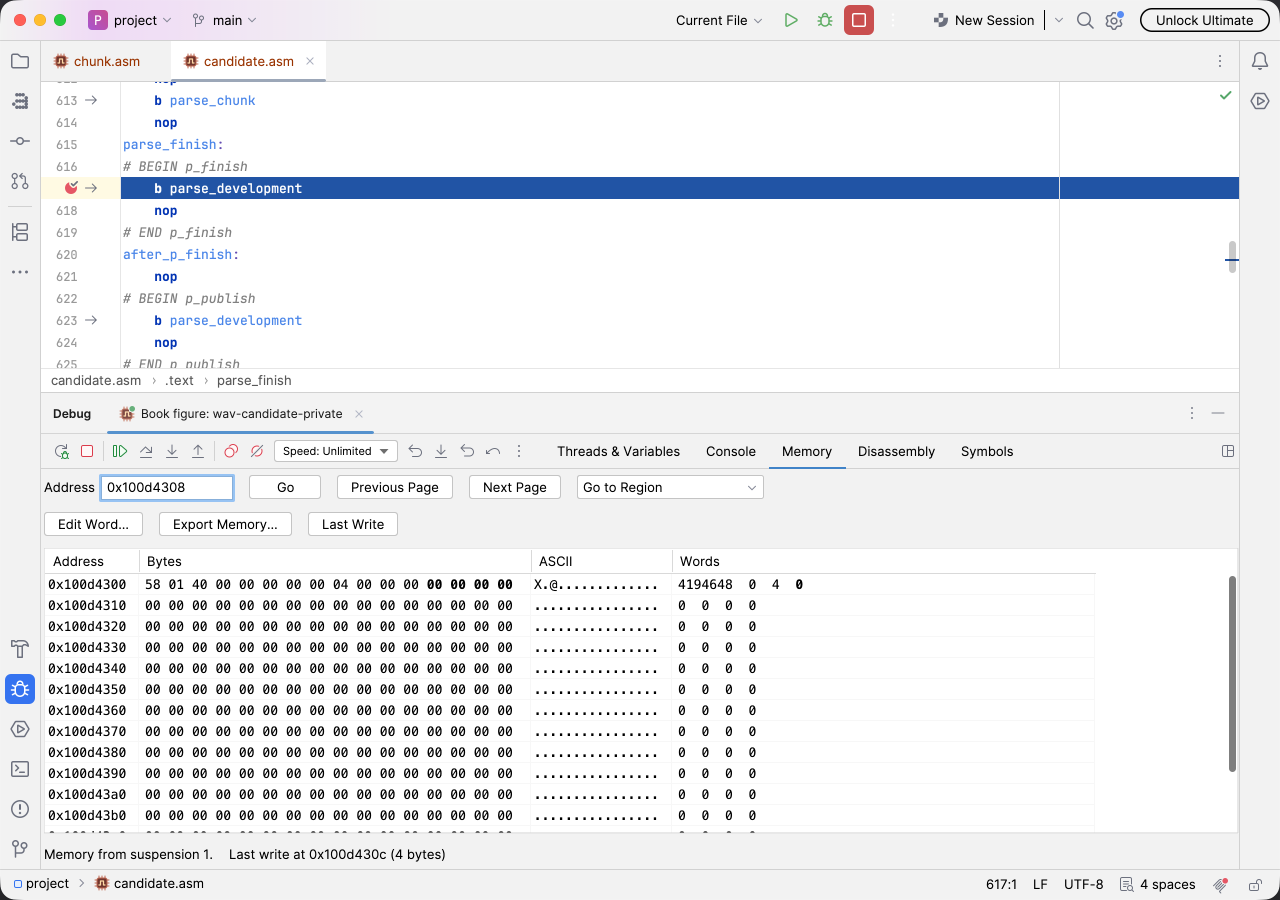
\includegraphics[artifact]{packages/031-pcm-wav/captures/f03/private.png}}
  \newsavebox{\MARSwavcandidatemetadataBox}
  \sbox{\MARSwavcandidatemetadataBox}{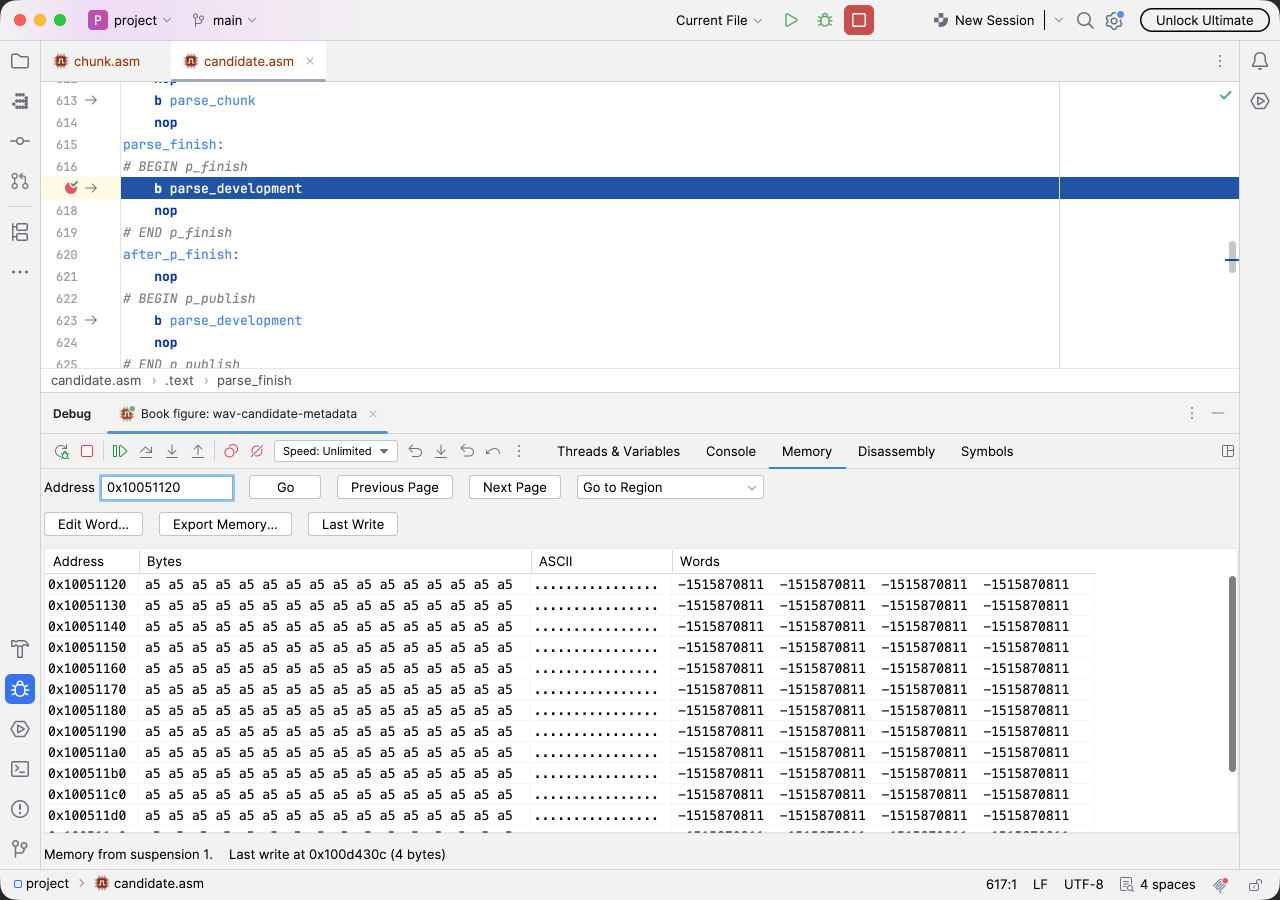
\includegraphics[artifact]{packages/031-pcm-wav/captures/f03/metadata.png}}
  \edef\MARSwavcandidatesourceLeft{\the\dimexpr0.036718750\wd\MARSwavcandidateregistersBox\relax}
  \edef\MARSwavcandidatesourceBottom{\the\dimexpr0.774444444\ht\MARSwavcandidateregistersBox\relax}
  \edef\MARSwavcandidatesourceRight{\the\dimexpr0.713281250\wd\MARSwavcandidateregistersBox\relax}
  \edef\MARSwavcandidatesourceTop{\the\dimexpr0.170000000\ht\MARSwavcandidateregistersBox\relax}
  \edef\MARSwavcandidatestateLeft{\the\dimexpr0.246093750\wd\MARSwavcandidateregistersBox\relax}
  \edef\MARSwavcandidatestateBottom{\the\dimexpr0.233333333\ht\MARSwavcandidateregistersBox\relax}
  \edef\MARSwavcandidatestateRight{\the\dimexpr0.553906250\wd\MARSwavcandidateregistersBox\relax}
  \edef\MARSwavcandidatestateTop{\the\dimexpr0.607777778\ht\MARSwavcandidateregistersBox\relax}
  \edef\MARSwavcandidatelengthLeft{\the\dimexpr0.246093750\wd\MARSwavcandidateregistersBox\relax}
  \edef\MARSwavcandidatelengthBottom{\the\dimexpr0.077777778\ht\MARSwavcandidateregistersBox\relax}
  \edef\MARSwavcandidatelengthRight{\the\dimexpr0.553906250\wd\MARSwavcandidateregistersBox\relax}
  \edef\MARSwavcandidatelengthTop{\the\dimexpr0.896666667\ht\MARSwavcandidateregistersBox\relax}
  \edef\MARSwavcandidateprivateLeft{\the\dimexpr0.034375000\wd\MARSwavcandidateprivateBox\relax}
  \edef\MARSwavcandidateprivateBottom{\the\dimexpr0.334444444\ht\MARSwavcandidateprivateBox\relax}
  \edef\MARSwavcandidateprivateRight{\the\dimexpr0.584375000\wd\MARSwavcandidateprivateBox\relax}
  \edef\MARSwavcandidateprivateTop{\the\dimexpr0.608888889\ht\MARSwavcandidateprivateBox\relax}
  \edef\MARSwavcandidatemetadataLeft{\the\dimexpr0.034375000\wd\MARSwavcandidatemetadataBox\relax}
  \edef\MARSwavcandidatemetadataBottom{\the\dimexpr0.311111111\ht\MARSwavcandidatemetadataBox\relax}
  \edef\MARSwavcandidatemetadataRight{\the\dimexpr0.584375000\wd\MARSwavcandidatemetadataBox\relax}
  \edef\MARSwavcandidatemetadataTop{\the\dimexpr0.608888889\ht\MARSwavcandidatemetadataBox\relax}
  \begin{tikzpicture}[alt={Five details at parse_finish show the unfinished acceptance instruction, cursor and limit both 82, both chunk flags, rate 16000, channels two, PCM offset 56, length 16, a private four-frame count, and unchanged metadata.}]
    \node[anchor=north west,inner sep=0,font=\small\bfseries] (source-title) at (6mm,0) {Before final acceptance};
    \node[anchor=north west,inner sep=0] (source) at ([yshift=-1mm]source-title.south west) {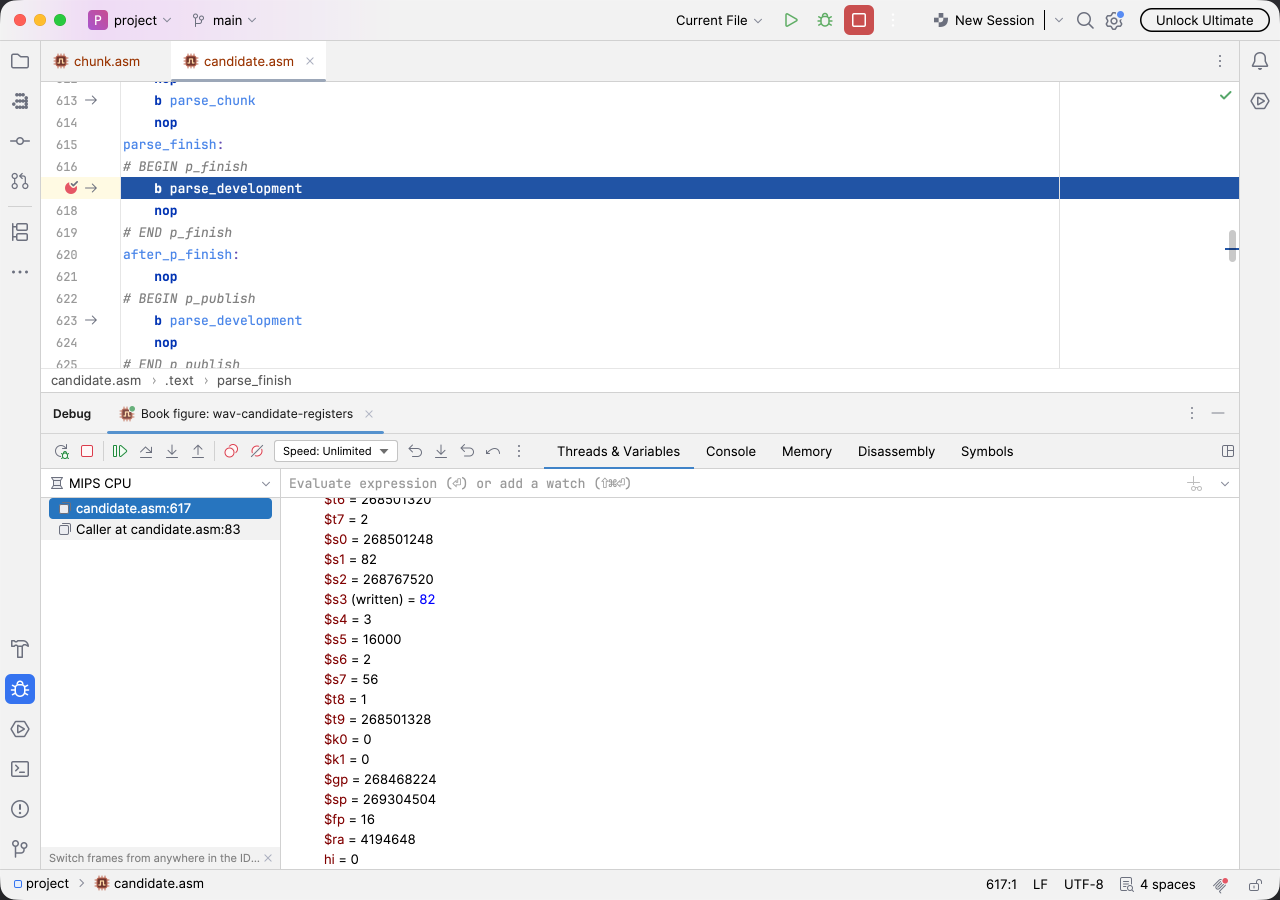
\includegraphics[width=0.54\linewidth,artifact,trim={\MARSwavcandidatesourceLeft{} \MARSwavcandidatesourceBottom{} \MARSwavcandidatesourceRight{} \MARSwavcandidatesourceTop{}},clip]{packages/031-pcm-wav/captures/f03/registers.png}};
    \begin{scope}[shift={(source.south west)},x={($(source.south east)-(source.south west)$)},y={($(source.north west)-(source.south west)$)}]
      \draw[black,line width=0.7pt] (0.237500000,0.080000000) rectangle (0.796875000,0.520000000);
      \node[draw=black,fill=white,circle,inner sep=1.5pt,font=\footnotesize] at ($(0.237500000,0.520000000)+(-3mm,0)$) {1};
    \end{scope}
    \node[anchor=north west,inner sep=0,font=\small\bfseries] (state-title) at ([yshift=-1mm]source.south west) {Container extent and retained candidate};
    \node[anchor=north west,inner sep=0] (state) at ([yshift=-1mm]state-title.south west) {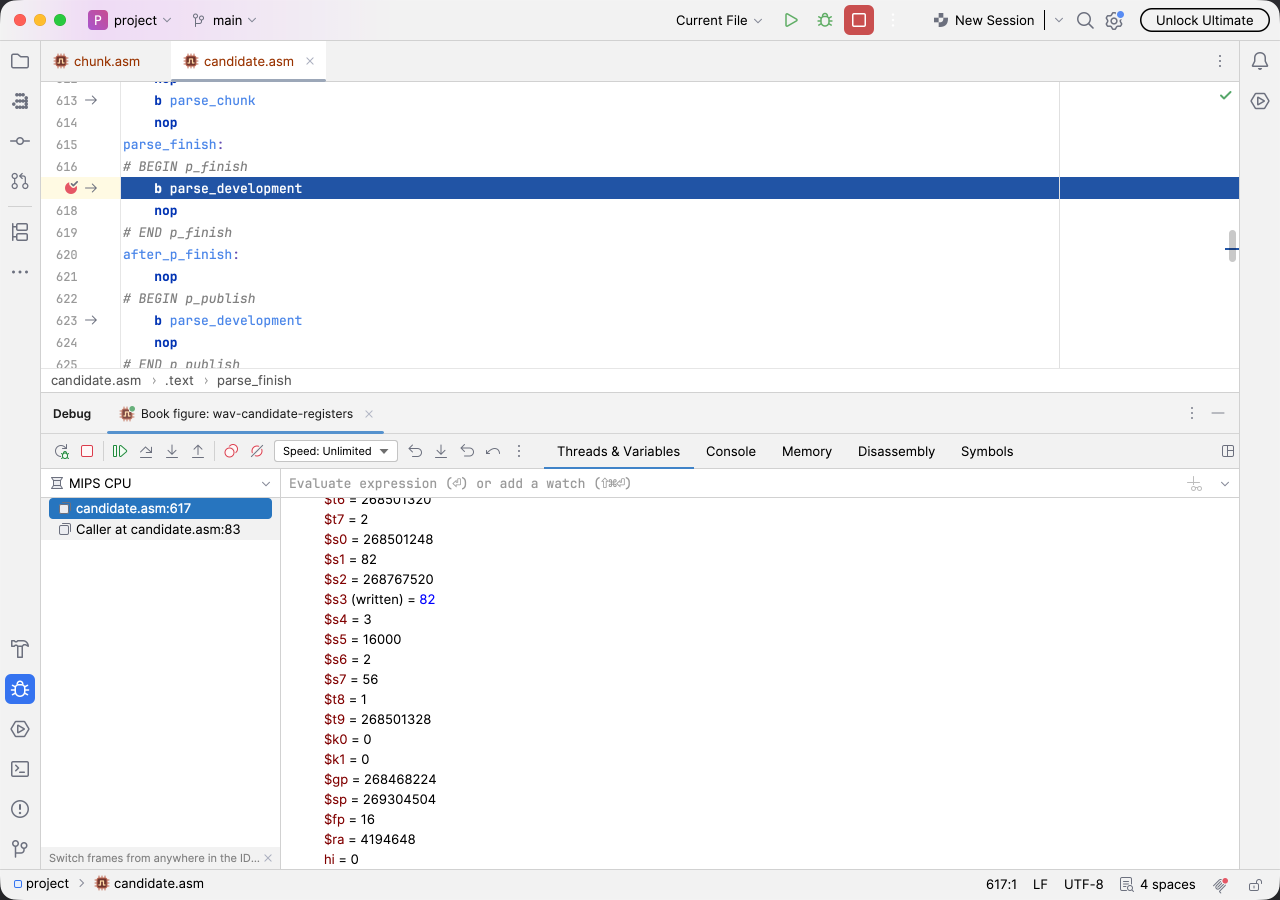
\includegraphics[width=0.48\linewidth,artifact,trim={\MARSwavcandidatestateLeft{} \MARSwavcandidatestateBottom{} \MARSwavcandidatestateRight{} \MARSwavcandidatestateTop{}},clip]{packages/031-pcm-wav/captures/f03/registers.png}};
    \begin{scope}[shift={(state.south west)},x={($(state.south east)-(state.south west)$)},y={($(state.north west)-(state.south west)$)}]
      \draw[black,line width=0.7pt] (0.023437500,0.006993007) rectangle (0.476562500,0.986013986);
      \node[draw=black,fill=white,circle,inner sep=1.5pt,font=\footnotesize] at ($(0.023437500,0.986013986)+(-3mm,0)$) {2};
    \end{scope}
    \node[anchor=north west,inner sep=0,font=\small\bfseries] (length-title) at ([yshift=-1mm]state.south west) {PCM byte length};
    \node[anchor=north west,inner sep=0] (length) at ([yshift=-1mm]length-title.south west) {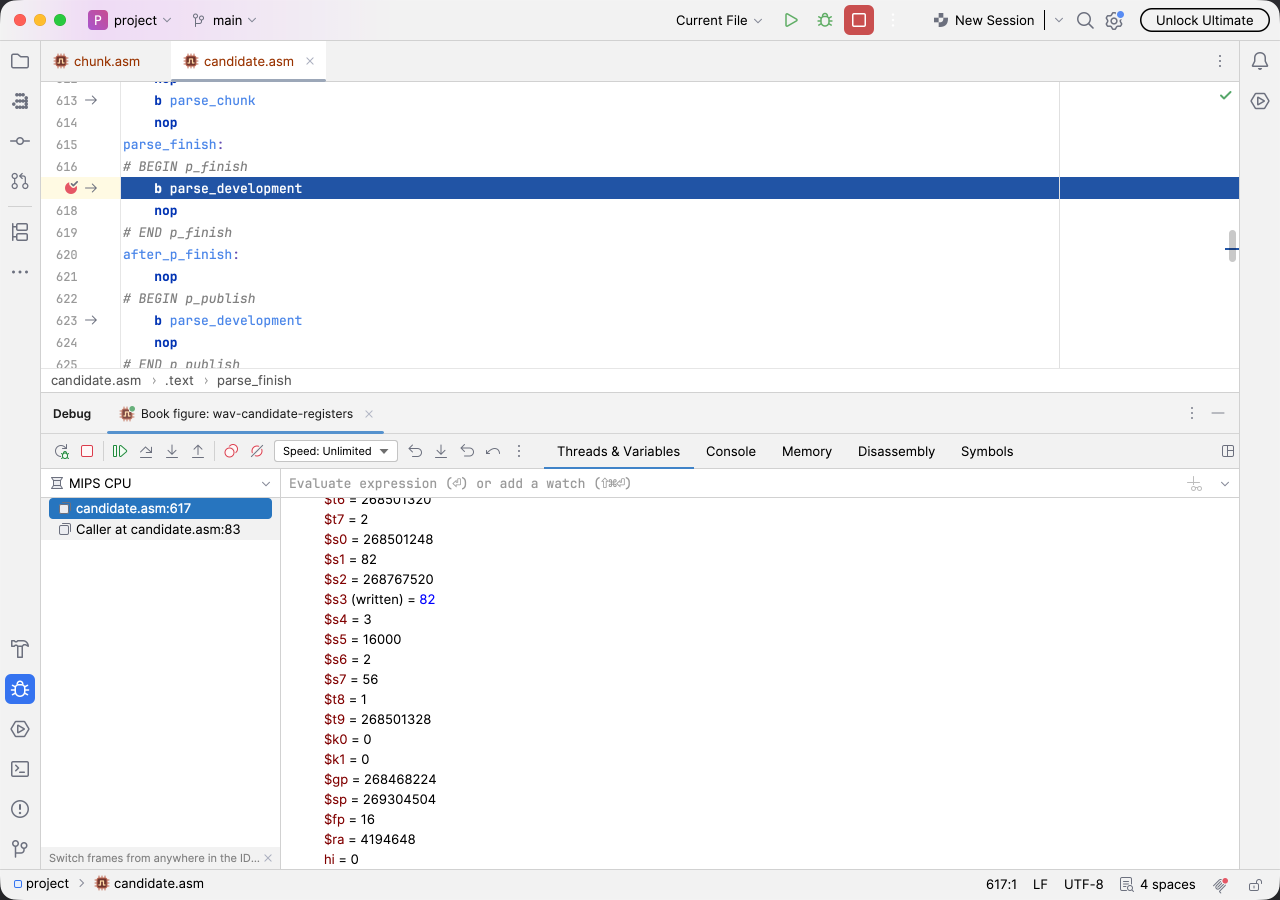
\includegraphics[width=0.44\linewidth,artifact,trim={\MARSwavcandidatelengthLeft{} \MARSwavcandidatelengthBottom{} \MARSwavcandidatelengthRight{} \MARSwavcandidatelengthTop{}},clip]{packages/031-pcm-wav/captures/f03/registers.png}};
    \begin{scope}[shift={(length.south west)},x={($(length.south east)-(length.south west)$)},y={($(length.north west)-(length.south west)$)}]
      \draw[black,line width=0.7pt] (0.023437500,0.043478261) rectangle (0.238281250,0.913043478);
      \node[draw=black,fill=white,circle,inner sep=1.5pt,font=\footnotesize] at ($(0.023437500,0.913043478)+(-3mm,0)$) {3};
    \end{scope}
    \node[anchor=north west,inner sep=0,font=\small\bfseries] (private-title) at ([yshift=-1mm]length.south west) {Private frame count beside the saved return address};
    \node[anchor=north west,inner sep=0] (private) at ([yshift=-1mm]private-title.south west) {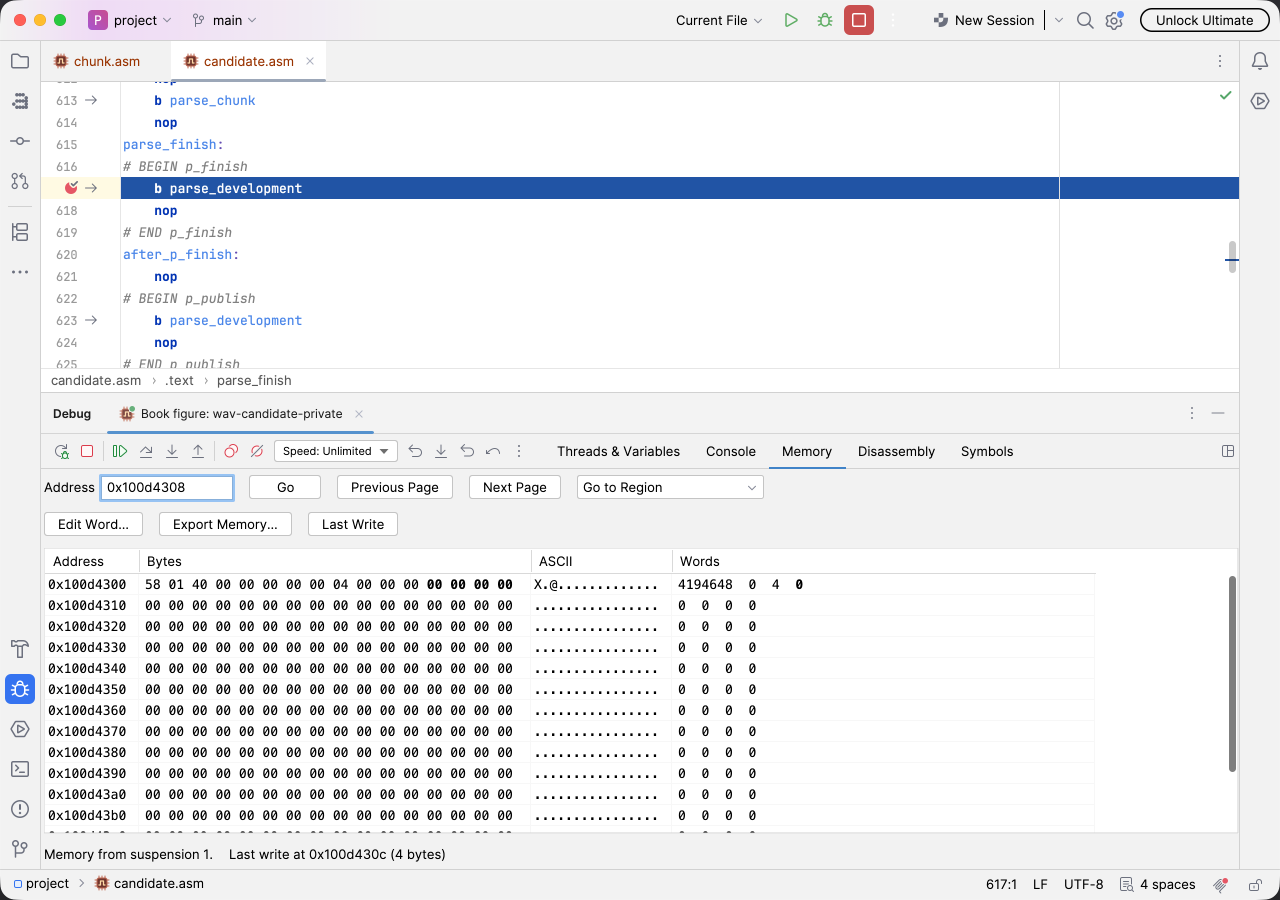
\includegraphics[width=0.84\linewidth,artifact,trim={\MARSwavcandidateprivateLeft{} \MARSwavcandidateprivateBottom{} \MARSwavcandidateprivateRight{} \MARSwavcandidateprivateTop{}},clip]{packages/031-pcm-wav/captures/f03/private.png}};
    \begin{scope}[shift={(private.south west)},x={($(private.south east)-(private.south west)$)},y={($(private.north west)-(private.south west)$)}]
      \draw[black,line width=0.7pt] (0.194672131,0.078431373) rectangle (0.997950820,0.490196078);
      \node[draw=black,fill=white,circle,inner sep=1.5pt,font=\footnotesize] at ($(0,0.490196078)+(-3mm,0)$) {4};
    \end{scope}
    \node[anchor=north west,inner sep=0,font=\small\bfseries] (metadata-title) at ([yshift=-1mm]private.south west) {Caller descriptor remains untouched};
    \node[anchor=north west,inner sep=0] (metadata) at ([yshift=-1mm]metadata-title.south west) {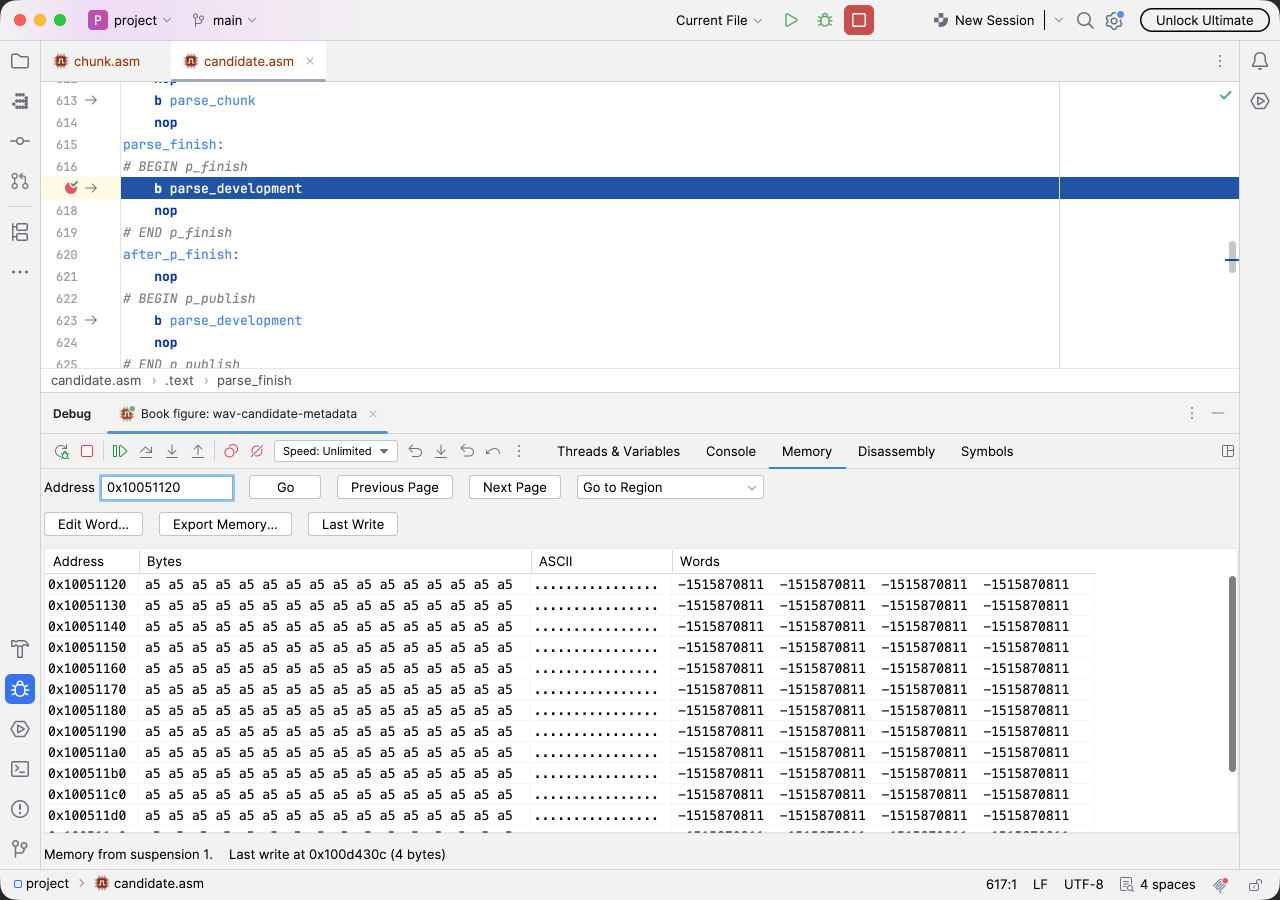
\includegraphics[width=0.84\linewidth,artifact,trim={\MARSwavcandidatemetadataLeft{} \MARSwavcandidatemetadataBottom{} \MARSwavcandidatemetadataRight{} \MARSwavcandidatemetadataTop{}},clip]{packages/031-pcm-wav/captures/f03/metadata.png}};
    \begin{scope}[shift={(metadata.south west)},x={($(metadata.south east)-(metadata.south west)$)},y={($(metadata.north west)-(metadata.south west)$)}]
      \draw[black,line width=0.7pt] (0.194672131,0.055555556) rectangle (0.997950820,0.638888889);
      \node[draw=black,fill=white,circle,inner sep=1.5pt,font=\footnotesize] at ($(0,0.638888889)+(-3mm,0)$) {5};
    \end{scope}
  \end{tikzpicture}
  \par\smallskip
  \begin{minipage}{\linewidth}
    \small
    \begin{enumerate}
      \setlength{\itemsep}{0pt}
            \setlength{\parsep}{0pt}
      \item The stop precedes final acceptance at \texttt{parse\_finish}. The chunk walk has reached the container end, but the finish and publication regions are still unfinished in this lesson stage.
      \item \texttt{s1 = s3 = 82} shows the limit and current offset. \texttt{s4 = 3} records both required chunks. The candidate retains rate 16000 in \texttt{s5}, two channels in \texttt{s6}, and PCM offset 56 in \texttt{s7}.
      \item \texttt{fp = 16} retains the PCM byte length. Dividing sixteen by four bytes per stereo frame gives four frames; the routine does not infer frame count from the total file length.
      \item The right-hand eight bytes of row \texttt{0x100d4300} hold the private frame count: \texttt{04 00 00 00 00 00 00 00}. They are at stack offset 80. The preceding eight bytes hold a saved return address, not another audio field.
      \item The displayed caller descriptor rows still contain \texttt{a5}. Its complete sixty-four-byte arena is checked unchanged. Final acceptance and publication will be authored next; retaining a candidate alone does not make a parse successful.
    \end{enumerate}
  \end{minipage}
  \caption{The parser retains a candidate before publishing the caller descriptor.}
  \label{capture:031-pcm-wav-f03}
  \label{pcm-wav-f03}
\end{figure}
\par
